%!TEX root = ../main.tex
%-------------------------------------------------------------------------------
\subsection{Economic framework}
%-------------------------------------------------------------------------------
EKW models describe sequential decision-making under uncertainty \citep{Gilboa.2009, Machina.2014}. At time $t = 1, \hdots, T$ each individual observes the state of the economic environment $s_t\in S$ and chooses an action $a_t$ from the set of admissible actions $\mathcal{A}$. The decision has two consequences: an individual receives an immediate utility $u_t(s_t, a_t)$ and the economy evolves to a new state $s_{t + 1}$. The transition from $s_t$ to $s_{t + 1}$ is affected by the action but remains uncertain. Individuals are forward-looking. Thus they do not simply choose the alternative with the highest immediate utility. Instead, they take the future consequences of their current action into account.

A policy $\pi = (a^\pi_1(s_1), \hdots, a^\pi_T(s_T))$ provides the individual with instructions for choosing an action in any possible future state. It is a sequence of decision rules $a^\pi_t(s_t)$ that specify the action at a particular time $t$ for any possible state $s_t$ under $\pi$. The implementation of a policy generates a sequence of utilities that depends on the objective transition probability distribution $p_t(s_t, a_t)$ for the evolution of state $s_t$ to $s_{t + 1}$ induced by the model. Individuals have rational expectations \citep{Muth.1961} so their subjective beliefs about the future agree with the objective transition probabilities of the model.

\autoref{Timing} depicts the timing of events in the model for two generic periods. At the beginning of period $t$, an individual fully learns about the immediate utility of each alternative, chooses one of them, and receives its immediate utility. Then the state evolves from $s_t$ to $s_{t + 1}$ and the process is repeated in $t + 1$.
%
\begin{figure}[b]
	%\vspace{1.0cm}
	\centering
	\scalebox{0.755}{	%!TEX root = ../main.tex

\definecolor{light-gray}{gray}{0.85}


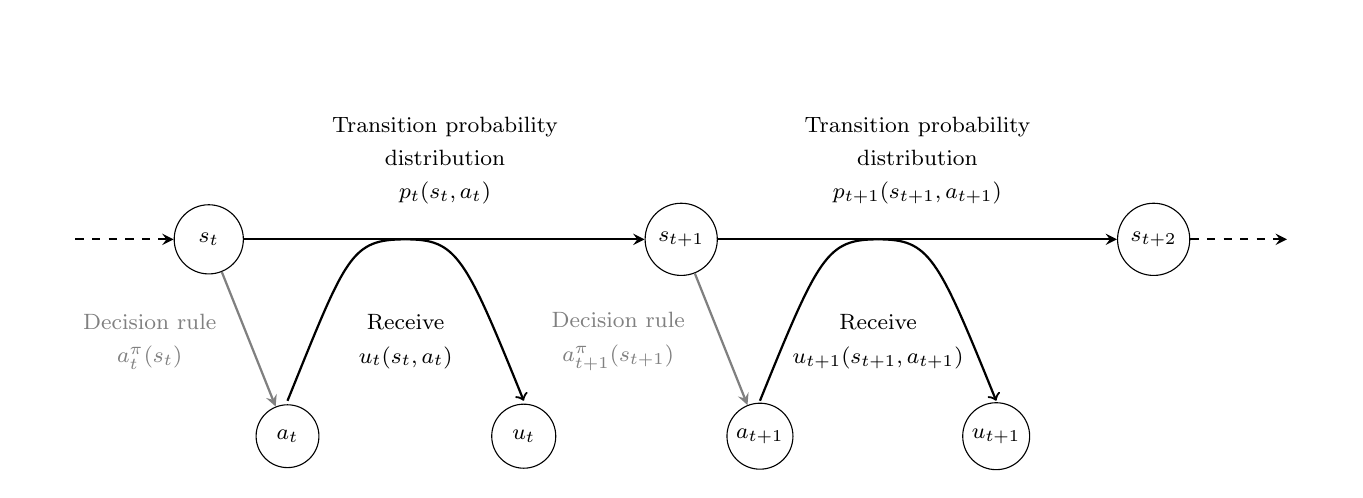
\begin{tikzpicture}[node distance=2cm]
%define styles
\tikzstyle{startstop} = [circle, rounded corners, minimum width=0.6cm, minimum height=0.3cm,text centered, draw=black]
[
->,
>=stealth',
auto,node distance=3cm,
thick,
main node/.style={circle, draw, font=\sffamily\Large\bfseries}
]
\tikzstyle{arrow} = [thick,->,>=stealth]]
\tikzstyle{darrow} = [dotted,->,>=stealth]]
%first and second column

\node (r0) [startstop, xshift = -3cm, draw = none] {}; 
\node (r999) [startstop, xshift = 13cm, draw = none] {}; 

\node (r1) [startstop, xshift = -1cm] {\footnotesize $~\,s_t\,~$};
\node (r2) [startstop, xshift = 5cm] {\footnotesize $s_{t+1}$};  %previously 4
\node (r3) [startstop, xshift = 11cm] {\footnotesize $s_{t+2}$}; %previously 8

\draw [arrow, dashed] (r0) -- node[anchor=south] {} (r1) ;
\draw [arrow] (r1) -- node[anchor=south] {} (r2) ;
\draw [arrow] (r2) -- node[anchor=south] {} (r3) ;
\draw [arrow, dashed] (r3) -- node[anchor=south] {} (r999) ;

\node (r4) [startstop, xshift = 0 cm, yshift = -2.5cm, inner sep = 0.08cm] {\footnotesize $~\,a_t\,~$ };
\node (r5) [startstop, xshift = 3 cm, yshift = -2.5cm, inner sep = 0.08cm] {\footnotesize $~\,u_t\,~$ };
\node (r6) [startstop, xshift = 6 cm, yshift = -2.5cm, inner sep = 0.08cm] {\footnotesize $a_{t+1}$ };
\node (r7) [startstop, xshift = 9 cm, yshift = -2.5cm, inner sep = 0.08cm] {\footnotesize $u_{t+1}$ };

\draw [arrow, color = gray] (r1) -- node[anchor=south] {} (r4) ;
\draw [arrow, color = gray] (r2) -- node[anchor=south] {} (r6) ;

\draw[ thick](0,-2.05).. controls (0.75, -0.2) and (0.8,0)..(1.5, 0);
\draw[->, thick](1.5, 0).. controls (2.15, 0) and (2.25, -0.2)..(3, -2.05);
\draw[ thick](6,-2.05).. controls (6.75, -0.2) and (6.85,0)..(7.5, 0);
\draw[->, thick](7.5, 0).. controls (8.15, 0) and (8.25,-0.2)..(9, -2.05);

\node(r8)[startstop, xshift = - 1.75cm, yshift = -1.3cm, draw =none, color = gray, align=center] {\footnotesize Decision rule \\ \footnotesize $a_t^{\pi}(s_t)$ };
\node(r9)[startstop, xshift= 4.2cm, yshift = -1.3cm, draw =none, color =gray, align = center] {\footnotesize Decision rule \\ \footnotesize $a_{t+1}^{\pi}(s_{t+1})$ };
\node(r10)[startstop, yshift = 1cm, xshift = 2cm, draw =none, align=center ] {\footnotesize Transition probability\\ \footnotesize distribution \\ \footnotesize $p_t(s_t, a_t)$};
\node(r11)[startstop, yshift = 1cm, xshift = 8cm, draw =none, align=center ] { \footnotesize Transition probability\\ \footnotesize distribution \\ \footnotesize $p_{t+1}(s_{t+1}, a_{t+1})$};
\node(r12)[startstop, yshift = -1.3cm, xshift = 1.5cm, draw =none, align=center ] {\footnotesize Receive\\ \footnotesize  $u_t(s_t, a_t)$ };
\node(r13)[startstop, yshift = -1.3cm, xshift = 7.5cm, draw =none, align=center ] {\footnotesize Receive\\ \footnotesize  $u_{t+1}(s_{t+1}, a_{t+1})$ };

\end{tikzpicture}
}
	\caption{Timing of events}
	\label{Timing}
\end{figure}
%
\noindent Individuals face uncertainty and they seek to maximize the expected total discounted utilities. An exponential discount factor ${0 < \delta < 1}$ parameterizes their time preference and captures a taste for immediate over future utilities.

Equation~\eqref{Objective Risk} provides the formal representation of the individual's objective. Given an initial state $s_1$, individuals implement the policy $\pi$ from the set of all possible policies $\Pi$ that maximizes the expected total discounted utilities over all $T$ decision periods given the information $\mathcal{I}_1$ available in the first period:
%
\begin{align}\label{Objective Risk}
	\max_{\pi \in\Pi} \E_{s_1}^\pi\left[\left.\sum^{T}_{t = 1}  \delta^{t - 1} u_t(s_t, a^\pi_t(s_t))\,\right\vert\,\mathcal{I}_1\,\right].
\end{align}
%
The superscript of the expectation emphasizes that each policy $\pi$ induces a different probability distribution over the sequences of utilities.
